% A poster using beamerposter and the gemini theme with epfl colors.
% Beamerposter will let you create a poster in a single beamer frame
% using the columns and blocks from the beamer class.
% The color theme is adapted from Gemini's MIT scheme.

% use beamer as documentclass
\documentclass[final]{beamer}

% use the beamerposter package to create a poster
\usepackage[scale=1.4,orientation=portrait,size=a0]{beamerposter}
\usepackage{csquotes}
\usepackage[backend=biber,giveninits=true,maxbibnames=99,bibencoding=utf8,style=numeric]{biblatex}
\addbibresource{references.bib}
% make references small
\renewcommand*{\bibfont}{\scriptsize}

% use the gemini theme.
\usetheme{gemini}
% use the epfl color theme, defining epflred, -darkgray,  -lightgray, -gray, and -blue
\usecolortheme{epfl}

\usepackage{graphicx}
\usepackage{tikz}
\usepackage{adjustbox}
\usepackage{qrcode}
\usepackage{wrapfig}
\usepackage{blindtext}

\newcommand*{\pianoroll}{
  \draw (0,2) rectangle (1,2.4);
  \draw (1,2.4) rectangle (2,2.8);
  \draw (2,2) rectangle (2.5,2.4);
  \draw (2.5,1.6) rectangle (3,2);
  \draw (3,1.2) rectangle (3.5,1.6);
  \draw (3.5,0.8) rectangle (4,1.2);

  \draw (4,1.6) rectangle (5,2);
  \draw (5,2) rectangle (6,2.4);
  \draw (6,1.6) rectangle (6.5,2);
  \draw (6.5,1.2) rectangle (7,1.6);
  \draw (7,0.8) rectangle (7.5,1.2);
  \draw (7.5,0.4) rectangle (8,0.8);

  \draw (1,-0.4) rectangle (2,0);
  \draw (2,0) rectangle (4,0.4);
  \draw (5,-0.8) rectangle (6,-0.4);
  \draw (6,-0.4) rectangle (8,0);
}

\newcommand{\sgcross}[1]
{
  \begin{scope}[xshift=#1cm,thick,color=epflred]
    \draw (0.35,0.1) -- (0.55,0.3);
    \draw (0.55,0.1) -- (0.35,0.3);
  \end{scope}
}
\newcommand{\sgbox}[1]
{
  \begin{scope}[xshift=#1cm]
    \draw (0,0) rectangle (0.9,0.4);
  \end{scope}
}
\newcommand{\sgboxfill}[2]
{
  \begin{scope}[xshift=#2cm]
    \draw[fill=#1] (0,0) rectangle (0.9,0.4);
  \end{scope}
}
\newcommand{\sgrow}[4][epflgray]
{
  \begin{scope}[yshift=#2cm]
    \foreach \x in {0,...,8} { \sgbox{\x} }
    \foreach \x in {#3} { \sgboxfill{#1}{\x} }
    \foreach \x in {#4} { \sgcross{\x} }
  \end{scope}
}

\title{Inferring Tonality from Note Distributions: \\ Why Models Matter}

\author{Fabian C. Moss\textsuperscript{\textasteriskcentered}, Martin Rohrmeier}

\institute{Digital and Cognitive Musicology Lab, École Polytechnique Fédérale de Lausanne}


\begin{document}

\begin{frame}[t]

  \begin{minipage}[t][.56\textheight][t]{\textwidth}

  \begin{columns}[t]
    \begin{column}{0.3\textwidth}
      \begin{block}{Background}
        Pitch-class statistics in pieces are assumed to correspond to mental representations of tonality \cite{Huron2006}.
      \end{block}

      \vspace{5em}

      \begin{block}{References}
          \printbibliography
      \end{block}

      \begin{block}{Acknowledgements}

        \begin{wrapfigure}{l}{.4\textwidth}
          
\includegraphics[width=.4\textwidth]{img/Logo_EPFL.pdf}
        \end{wrapfigure}

        \small
        The research presented on this poster is generously
        supported by EPFL through the Latour Chair in Digital Musicology.
      \end{block}
    \end{column}

    \begin{column}{0.3\textwidth}
      \begin{block}{Improvement 1}
        Use models of tonal pitch space to reveal further regularities in pitch-class distributions \autocite{Harasim2019}
      \end{block}

      \begin{block}{Improvement 2}
        \blindtext
      \end{block}

    \end{column}

    \begin{column}{0.3\textwidth}
      \begin{block}{Basic Algorithm}
        The algorithm for enumerating skipgrams takes as input:

        \begin{itemize}
        \item a list $L$ of objects to generate skipgrams over
        \item a skip function $f$ on pairs of objects
        \item the skipgram length $n$
        \item the skip limit $k$
        \end{itemize}

        The list $L$ must be ordered with respect to the skip function:
        \[\forall i < j < k: f(L_i,L_j) \leq f(L_i,L_z).\]

        The algorithm returns all sublists $x$ of $L$ with $|x| = n$ and
        $\sum_i f(x_i,x_{i+1}) \leq k$.

        $L$ is traversed, building up a \alert{list of prefixes}
        that eventually become complete skipgrams.

        For each element $e$ in $L$:
        \begin{enumerate}
        \item remove old prefixes that cannot be extended with $e$
        \item extend all remaining prefixes with $e$%; of those:
          %\begin{enumerate}
          \item output all completed prefixes (length $n$)
          \item add all incomplete prefixes to the prefix list
          %\end{enumerate}
        \item add a new prefix $[e]$.
        \end{enumerate}

        \begin{adjustbox}{scale=2,center,margin=0 1ex}
          \begin{tikzpicture}
            \begin{scope}[scale=0.3]
              \pianoroll
              \draw[fill=epflgray] (1,-0.4) rectangle (2,0);
              \draw[fill=epflgray] (2,2) rectangle (2.5,2.4);
            \end{scope}

            \begin{scope}[scale=0.3,yshift=4cm]
              \fill[epfllightgray] (-0.25,-1) rectangle (8.25,3);
              \pianoroll
              \draw[fill=epflred] (0,2) rectangle (1,2.4);
              \draw[fill=epflred] (2,2) rectangle (2.5,2.4);
            \end{scope}

            \begin{scope}[scale=0.3,yshift=8cm]
              \pianoroll
              \draw[fill=epflgray] (1,-0.4) rectangle (2,0);
              \draw[fill=epflgray] (1,2.4) rectangle (2,2.8);
            \end{scope}

            \draw (2.75,-0.4) -- (2.75,3.2);

            \begin{scope}[xshift=3cm,yshift=0.4cm]
              \pianoroll
              \draw[fill=epflgray] (0,2) rectangle (1,2.4);
              \draw[fill=epflgray] (2,2) rectangle (2.5,2.4);
              \draw[fill=epflred] (3,1.2) rectangle (3.5,1.6);
            \end{scope}
          \end{tikzpicture}
        \end{adjustbox}
      \end{block}

      \begin{block}{Extensions}
        Efficient \alert{filtering} can be implemented
        by \alert{testing a predicate} on every extension of a prefix.
        If the new prefix does not satisfy the predicate, it is discarded.

        \alert{Sampling} can be implemented efficiently
        by \alert{flipping a coin} on every prefix extension,
        deciding whether to keep or to discard the prefix.
        A prefix is extended $n-1$ times,
        so keeping each prefix with probability $\sqrt[n-1]{p}$
        means keeping the skipgram with probability $p$.

        The output order depends on the last element of each skipgram,
        because the algorithm outputs skipgrams when they are completed.
        If the \alert{order of the initial elements} should be retained,
        completed skipgrams are first entered in a \alert{priority queue}.
        In each iteration, only those skipgrams are taken from the queue
        that cannot be preceded by currently active prefixes anymore.
      \end{block}

    \end{column}
  \end{columns}

\end{minipage}

\begin{minipage}[t][.3\textheight][t]{\textwidth}
  \begin{block}{Historical Development}

    \begin{figure}
      \centering
      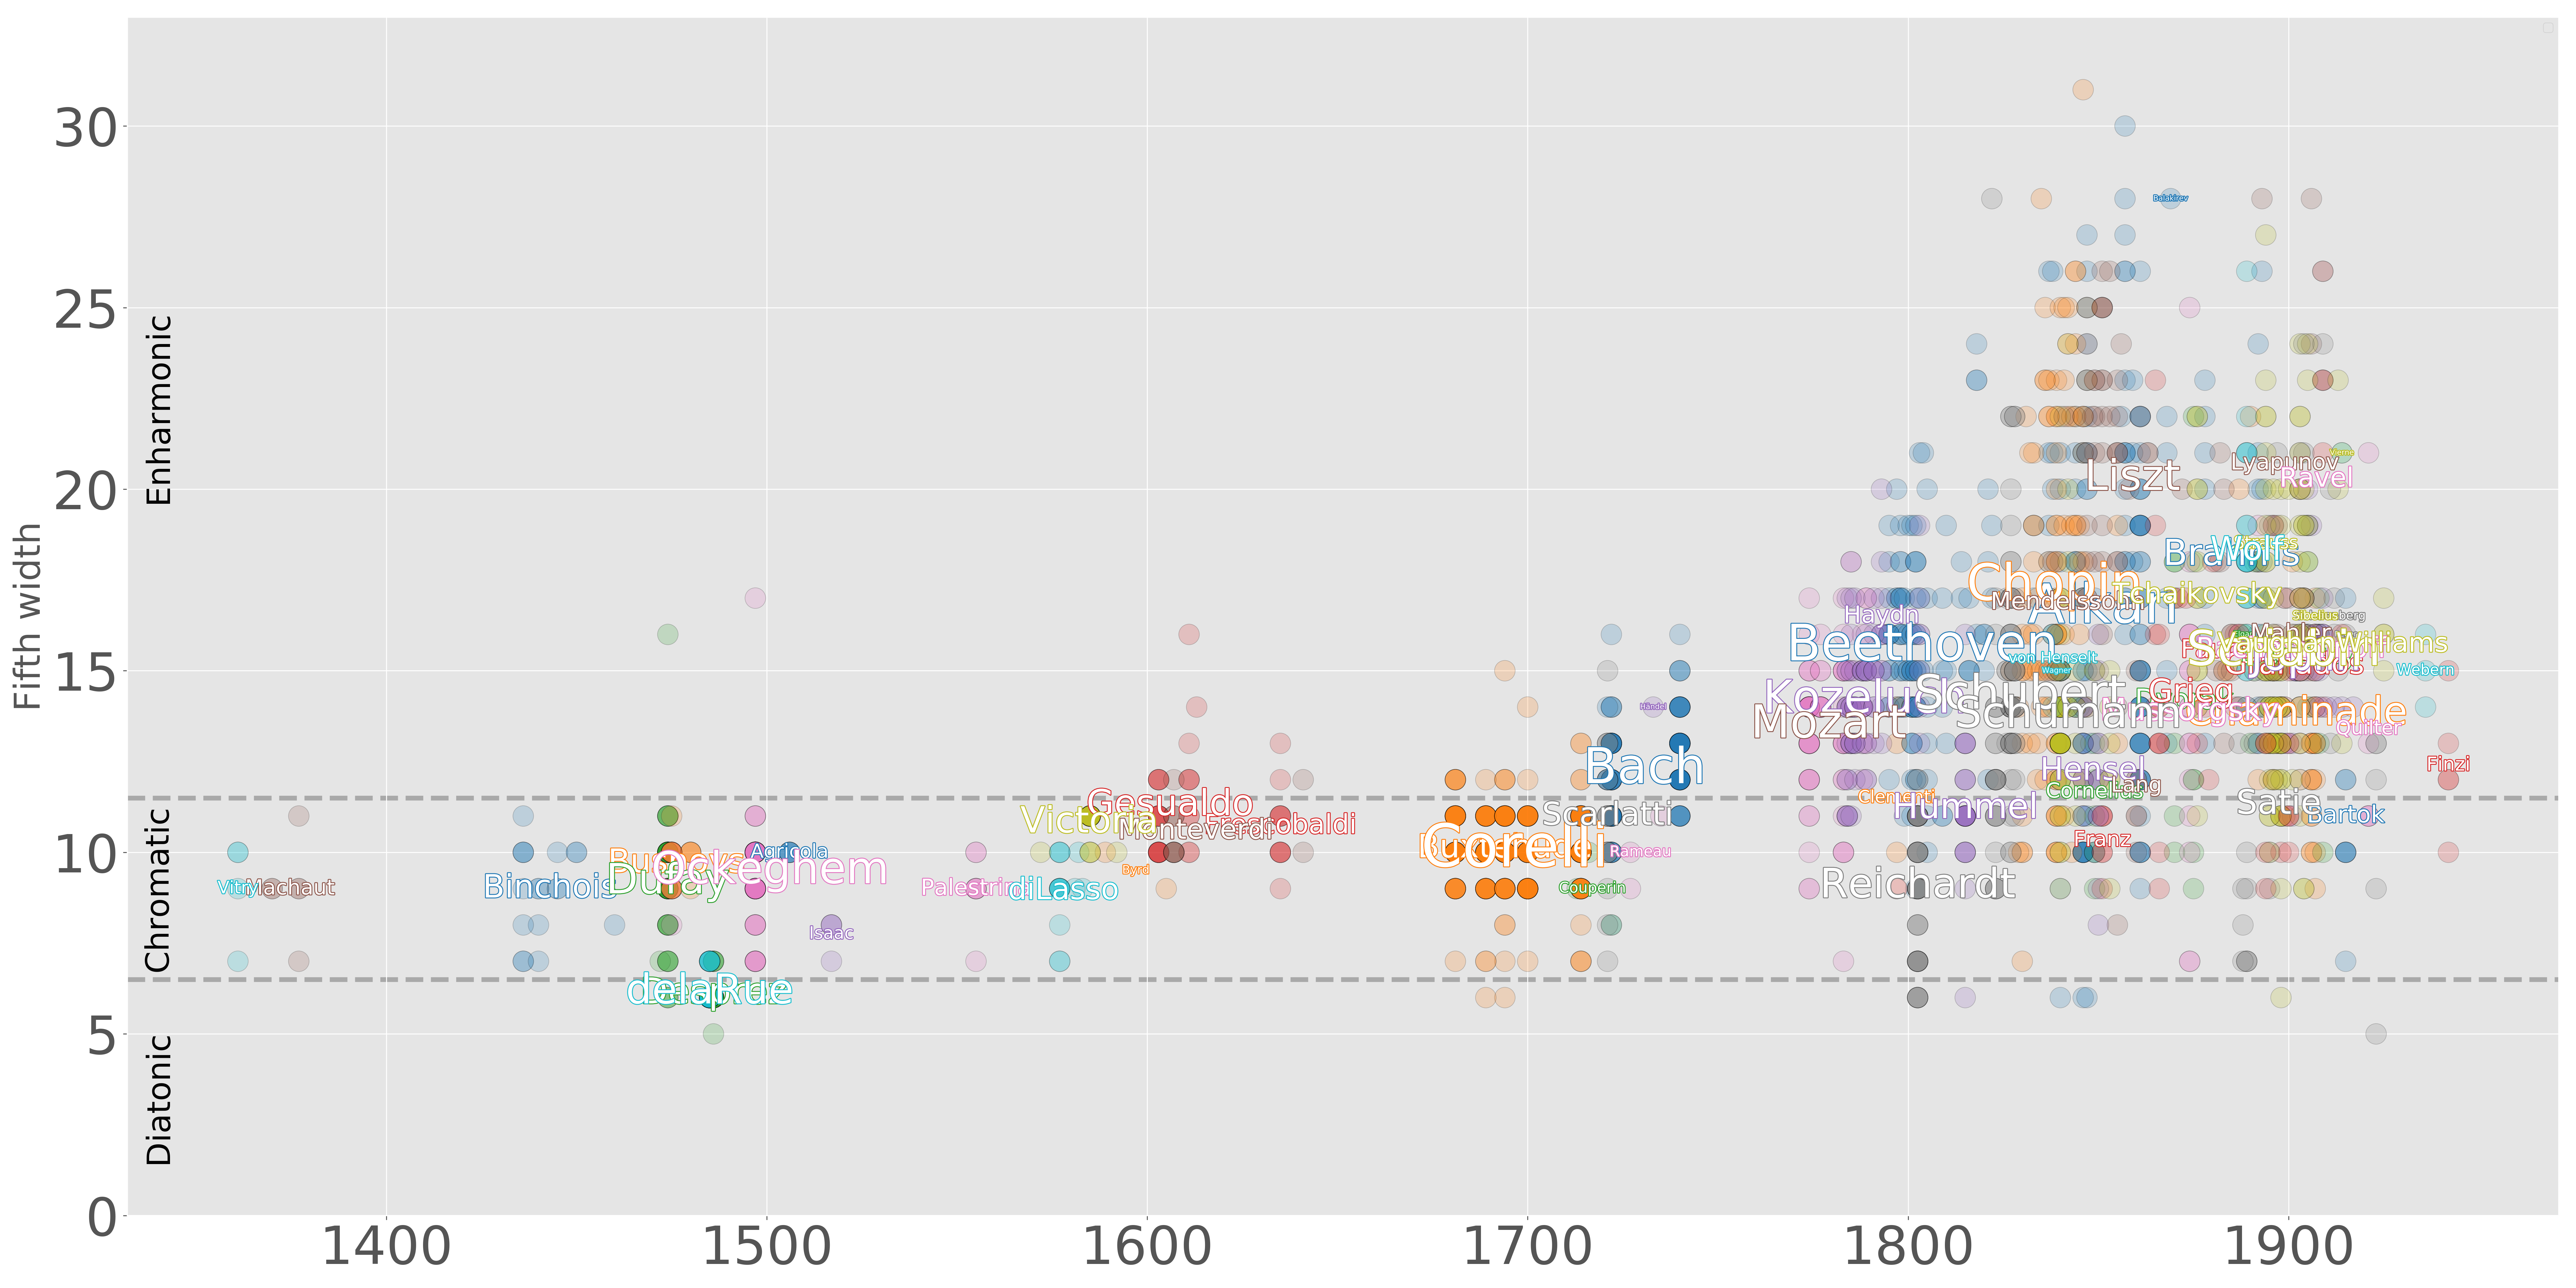
\includegraphics{img/fifth_widths}
      % \caption{}
      % \label{}
    \end{figure}

  \end{block}
\end{minipage}

\end{frame} % End of the enclosing frame

\end{document}
